\begin{figure}[htpb]
	\centering\capstart{}
	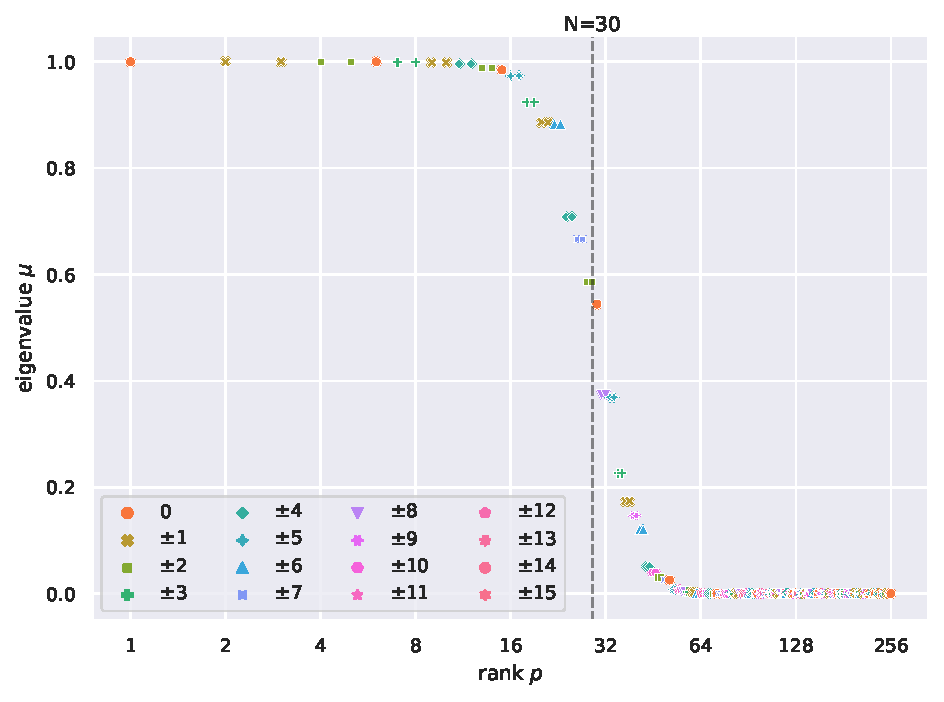
\includegraphics[width=\textwidth]{polar_cap_eigenvalues.pdf}
	\caption[
        The Slepian eigenvalues within a \(\SI{40}{\degree}\) polar cap
	]{
        The ordered Slepian eigenvalues within a polar cap of colatitudinal radius \(\SI{40}{\degree}\).
        The bandlimit here is  \(L=16\), which corresponds to a Shannon number of \(N=30\), as indicated on the plot.
        Most of the eigenvalues are \(\almost{1}\) before decreasing rapidly towards zero around the Shannon number.
        The different symbols represent the orders \(-15 \leq m \leq 15\), where adjacent matching symbols are \(\pm m\) doublets.
	}\label{fig:chapter2_polar_cap_eigenvalues}
\end{figure}
